%
% Copyright (c) 2011 Betti Österholz
%
% Permission is granted to copy, distribute and/or modify this document
% under the terms of the GNU Free Documentation License, Version 1.2 or
% any later version published by the Free Software Foundation;
% with no Invariant Sections, no Front-Cover Texts, and no Back-Cover Texts.
%
% A copy of the license is included in the file ``fdl.tex'' .
%

%path for pictures
\graphicspath{{./stock_environment/}}
\graphicspath{{./stock_environment/}{../stock_environment}}


\newpage
\part{The genetic algorithm}\index{genetic algorithm}\index{algorithm}
\label{secGeneticAlgorithmDesign}

In this section, general design decisions and initial analysis for the genetic algorithm are established.
The realized genetic algorithm is flexible and expandable designed.

The genetic algorithm is also an evolutionary algorithm. The term ``genetic'' refers to the ability of the algorithm to encode information of two or more individuals in a new individual and that it is working on information that code the (multimedia) object and do not represent those objects directly.

The algorithm is used to generate Fib objects, which represent a multimedia object as well as possible. The algorithm is given a particular multimedia object, for that it generates Fib objects /individuals, of which good will be selected. The creation of new individuals may also include analysis of the multimedia object and the use or analysis of information from other individuals. Which individuals are good, can be decided by the given parameters (by the evaluator for individuals).

\bigskip\noindent
The algorithm consists of five separate parts:
\begin{itemize}
 \item the core algorithm
 \item the evaluator for individuals
 \item the mortality rating algorithm
 \item the evaluator for operators
 \item the set of operators
\end{itemize}

In Figure \ref{figGeneticAlgorithmus} a sketch for the flow diagram for the genetic algorithm is shown.

\begin{figure}[htbp]
\begin{center}
  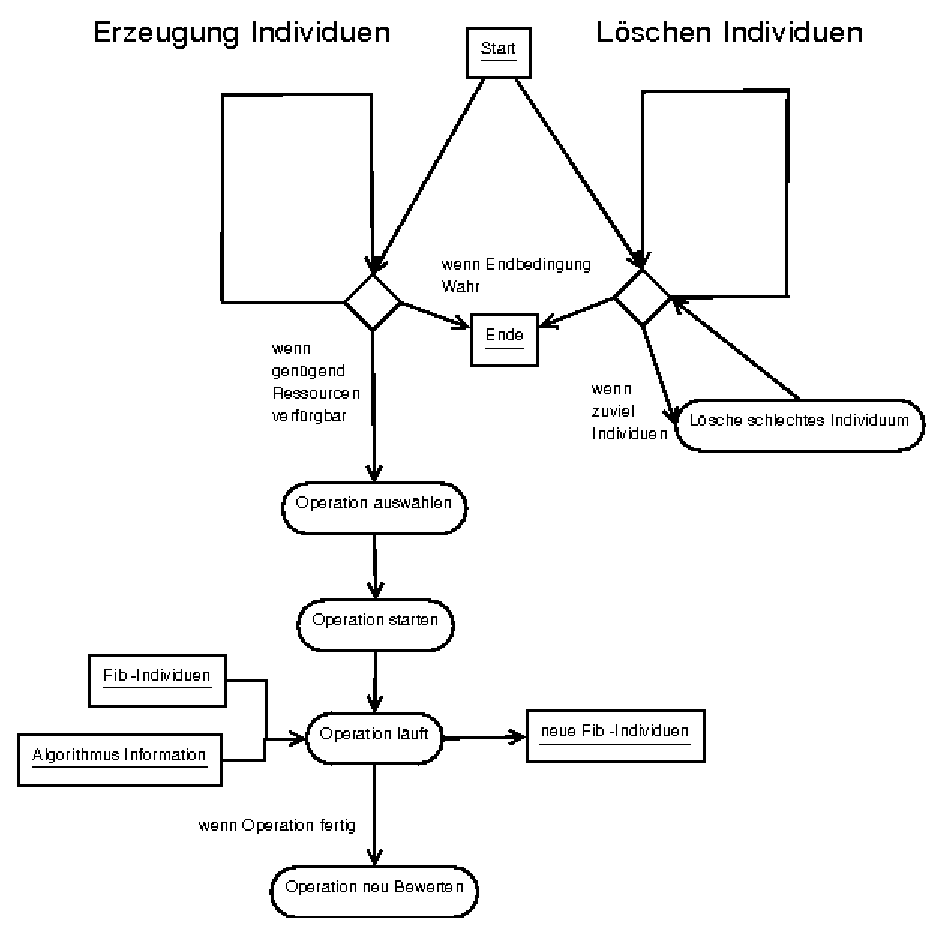
\includegraphics[scale=0.4]{algorithmus}
\end{center}
\caption{Flow diagram of the genetic algorithm}
\label{figGeneticAlgorithmus}
\end{figure}

In the following the single Fib objects are called individuals. The set of all individuals, who are existing at a time in the algorithm, is calle population.


\section{Core algorithm}\index{core algorithm}

The core algorithm uses the evaluator and the operators to realize the genetic algorithm. It is simple and flexible.

The evaluators for individuals or operators are (with the help of parameters) interchangeably.

\bigskip
The core algorithm includes the main loop of the genetic algorithm, which calls the operators and generates the individuals.

The second loop in the algorithm is the selection loop. It will delete individuals.

\bigskip
In addition, the core algorithm provides functions for the operators. The operators are called by the core algorithm through a method, that is the same for all operators. After that, the operators can get, with the help of the functions of the core algorithm, the algorithm specific values, e. g. such as individuals, which the operations will use. In this way, the operators will always look the same in each case for the core algorithm, and the core algorithm does not need any logic specific to a particular operator. Thereby future adjustments to the operators are simplified, because not the interface of all operators have to be be adjusted, but only the functions, which are provided by the core algorithm.

The calling method for the operators should be flexible, so that operators can be started concurrently and the algorithm don't have to wait for the completion of each operation. The operators should be run separately from the core algorithm and affect it only by the specified interface. A faulty operator should not lead to errors in or termination of the entire system.


\section{Evaluator for individuals}\index{evaluator!individuals}

The concrete evaluator algorithm should be simple to replace, so it can be adapted to various problems. The respective evaluation algorithm is needed to calculate the fitness of an individual.

With the help of parameters for special evaluators, they can be further adjusted (for example it can be adjusted, how important a small size compared to a fast evaluation of individuals is).


\subsection{The fitness of individuals}\index{fitness!individuals}

The fitness of an individuals is determined by different fitness factors.

One of the most important is, to what extent the individual is similar to the desired original multimedia data (such as the original image). The more the individual (or the phenotype of it) is similar to the original multimedia data, the higher the fitness should be and the lower is the error, which the individual has for the display of the original multimedia data.

This error (and thus the fitness of the individual) can be determine for example, with the sum of (the squared) differences (not defined points give the maximum error) of the colors of the points between the original image and the image produced by the individual, or through another self-determined distance.

If the fitness of separate part objects of the individual should be determined, this can be achieved, for example, by including in the evaluation only the area that is covered by the part object, the covered area and a border around this area or only the smallest square, which encompass this part object.

Another useful fitness factor is the size (increases with the number of elements) of the separate individuals, to give bigger individuals a lower fitness than smaller individuals, with the same error on the original multimedia data, and to prefer the smaller individuals.

A further fitness factor, which can be included, is the estimate of the time it takes to evaluate the individual for displaying the multimedia object (phenotype). In this way maybe even the execution speed of the algorithm can be increased.


\subsection{Selection by deletion of individuals}\index{Selection}

In order to spare the resources (memory, CPU time), it is necessary to limit the number of individuals (Fib objects) in the working process (individuals wich participate in the genetic algorithm). Therefore (if required) individuals have to be removed from it. In this process individuals with lower fitness are preferred.

There is therefore a \textbf{mortality rating algorithm}\index{mortality} for the algorithm. It determines the probability, with which a individual is deleted. To delete individuals, there is a separate loop in the algorithm, in which is tested, whether the maximum number of individuals is exceeded. If this is the case, individuals will be deleted, until the number of individuals is back on track (lower the maximum number of individuals). In this case individuals with a high mortality assessment by the mortality rating algorithm have a high probability of being deleted.

The mortality assessment is based on the assessment of the fitness of individuals. However, the mortality rating algorithm can be exchanged for other mortality algorithm or be controlled by parameters. For example, it is possible to declare some individuals to be immortal, so they can not be deleted. By declaring, for example, the $n$ ($n>0$) best individuals to be immortal, it can be avoided, that they will be deleted and thus that one of the best individuals will be lost.

The mortality algorithm can furthermore access via the operator interface the status information of the genetic algorithm, to determine, for example, the number of previously generated individuals.


\section{Evaluator for operators}\index{evaluator!operators}

To determine which operator to selected next, they are evaluated. Operators, which are rated better in a situation, have a higher probability of being selected respectively run in a similar situation.

\bigskip\noindent
The situation may include:
\begin{itemize}
 \item how many operations wher executed.
 \item of which nature the original multimedia object is (with the help of the domains for the environment in the root-elements of it):
 \begin{itemize}
  \item it contains colors
  \item it is monochrome
  \item it contains sound
  \item it is a film
  \item ...
 \end{itemize}
 \item the average (relative) fitness of individuals.
 \item the fitness of the best/worst individual.
 \item the standard deviation of fitness values in the population.
 \item the number of individuals.
 \item the operations that have been executed.
 \item ...
\end{itemize}

The different evaluation algorithms can be selected. Thus, different evaluation algorithms can be easily interchanged and compared.

To evaluate the operators, data of their previous execution may be kept permanently (by the seperate evaluators). In this way, the algorithm can learn from previous operator calls.

The evaluation of the operators should be system independent, ie. independent of the computer, on which the algorithm is running.

\bigskip\noindent
The evaluation criteria can be:
\begin{itemize}
 \item execution time of the operation
 \item reached deterioration or improvement
 \item reliability of the operator (Is always a result returned? Did it crashes sometimes?)
 \item ...
\end{itemize}


\section{The genetic operators for Fib}

The operators are to be seen separately from the genetic algorithm. It should be possible to add any number of operators for the use in the genetic algorithm, without having to adjust it.

Each operator has a unique identifier or ID, through which related values (such as its performance to date) can be associated to it.

An running operator is called operation.

The operations are intended to implement coding algorithms. Operators should therefore not be as simple as possible, but may as well involve complex algorithms.

The operators should also be numerous, and the algorithm is responsible for the selection of good operators. Therefore, it is also desirable to create own operators with good parts of other operators. In this case, both the original operators and the new operator, which contains the extracted parts, should be in the genetic algorithm.

For special applications, a genetic algorithm may be used, which set of operators was restricted to the most useful operators for this application.
Also, for a application useful operators can be combined to a (not genetic) algorithm, that uses them in determinated way.


\subsection{Reproduction}

In the general ``reproduction'', a individual is choosen from the population, preferably a individual with an high fitness, than it is copied and modified by one operation. At the end it is added to the population. It can also be checked, if it is a ``new'' object (if there is no equal object in the population) and just added in this case, so there are no duplicate individuals in the population.

In the algorithm the reproduction is implemented by running an operator. This operation retrieves all the required data with the help of the operation interface of the algorithm. This required data may include one or more individuals or data on the recent course of the algorithm (e. g. the number of previous interactions respectively operations).


\section{The social aspect of the genetic algorithm}\index{algorithm!social aspect}

The strict separation of the operators from the algorithm and the ability to easily add operators, has its roots in rather social considerations.

Normal coding algorithms are limited to the encoding methods of one or a few ideas of some (in the order of 1 to 100) people (the development team). But there are world wide much more people (on the order of probably 100000) who deal in a broader sense with efficiently and easy encoding of multimedia objects, thereby inevitably many ideas to code multimedia objects remain ignored. Even if some of these people have an interested in contribute their ideas, this is very difficult or impossible to realize.

Everyone can contribute new ideas to the Fib algorithm in the form of new operators (a term for this is ``crowdsourcing''). To do this, it is sufficient to only possess the knowledge for the Fib multimedia description language and the interface for the operators of the algorithm. In order to introduce new ideas or operators, for efficiently coding of multimedia objects, no adjustments to the algorithm or other operators should be required. This will limit side effects and any implementation of an idea has only to worry about the idea respectively its operator. So there are no further knowledge needed of the algorithm or even other operators. In this way the system can grow, without increasing the complexity of the (base) system and with this the difficulty for maintenance and expansion of the system.

The algorithm and the image description language should be designed so that layman can train themself without much effort to implement new ideas respectively operators. In particular for students in computer science (or people with computer science as their hobby), it should be possible to train themself within a few days, so that they can implement their own operators and integrate them. (How useful or effective this is, should be of no concern here.)

The GNU GPL license, under which the algorithm is published, clarifies the legal situation for new operators. This allows to add new operators to the algorithm, unless other rights are infringed (an injury would be, for example, that the operators use an algorithm or code which are under incompatible licenses). New operators can also be made available to the public.

The rating of the operators should motivate people to integrate their own operators. Thus, anyone who has added an operator can realisticly assess, how good his operator is in relation to other operators in a situation. Competition among operator authors should be beneficial to the creation of new and better operators.

All this should result in that not only a small development team will contribut to improve the encoding of Fib objects, but that a much larger group of people are concerned with this issue. This should give the development and propagation of Fib a further boost.

In this sense, the genetic algorithm for Fib is a trans ingenious algorithm, that is designed to extract the ideas of people to encode multimedia data from their heads and then transport/collected them into one pool. Thus, these ideas/algorithms can accomplish more than they could individually. The algorithm can thus combine more intelligence than one human (or a small group) can produce.


\section{Why genetic algorithms are good for encoding multimedia objects}

There is, in general, no algorithm for converting raster graphics directly into memory-friendly vector images, where the strengths of the vector description language are actually used. For the conversion from one multimedia format into another, there is often a similar problem, especially when in the first multimedia format, the properties of points of a euclidean (discrete) space are given directly (for example, to be able to store images directly) and the second multimedia format encodes the multimedia objects with complex objects (such as rectangles and / or circles).

Since a genetic algorithm has the potential to generate all possible descriptions in a multimedia language and among these, of course, also good descriptions will be, that use the strengths of multimedia language in respect of the original object, a genetic algorithm has also the potential to generate good descriptions. If existing knowledge was well implemented into genetic algorithm, it can find good descriptions probably faster than a pure random search.

Yet another advantage of genetic algorithms is the great freedom in the choice of problem description (multimedia language) and the possible operators on it. This allows complete freedom to design a multimedia language according to your own ideas, wich has certain properties, such as readability or simplicity. Into the operators arbitrarily much knowledge can be incorporated. It is, for example, possible to use known good algorithms (e. g. to translate raster images into vector images) or parts of them in operators, so that the result from the genetic algorithm (on raster images) is at least as good as the algorithm, but even better results can be generate.

The major disadvantage of genetic algorithms that they need very much time or computing time is weakened by the fact, that this high initial cost can be ``cheap'' and pays off later. The genetic algorithm can run, for example, as a background process with low priority, so that it consumes superfluous processing power. Later, with the result that it has supplied, much bandwidth can be saved.

This all suggests to use genetic algorithms to encoding multimedia objects.


\section{Complexity estimation}
\label{abschaet}

%TODO secPowerOfFibOnPictures not existing
With the approach of section \ref{secPowerOfFibOnPictures} on page \pageref{secPowerOfFibOnPictures}, it is possible to converted an arbitrary raster image into an Fib object, with a computing time growing linearly to the number of points and ther properties, as each point and its properties can be easiely added to a list element and the required time for the creation of the other Fib elements (of the root-element) can be performed in constant time.

This approach can be extended to any multimedia data, which are represented as properties of points of a finite, euclidean and discrete space. Thus always an operator can be constructed, that converts a multimedia object in linear time with the number of points and properties into a corresponding Fib object. This Fib object grows only linearly in size with the number of points and ther properties of the original multimedia object.
This operator, however, doesn't produced good Fib object representations, because it does not use the possibilities of Fib.

How much effort is required to produce better Fib objects, is very difficult to estimate, since both the operators and the multimedia objects can be arbitrary. However, it can be assumed that, for multimedia objects with simpler structures the effort is lower.


\section{Analogy to the natural evolution}

As an analogy to the natural evolution strains of bacteria (e. g. E. coli) are used here. They have genes, on wich basis genetic evolution occurs in them.

In these bacterial strains (e. g. E. coli) gene transfer is possible, whereby some of the genetic information (genetic material or its copies) of one bacterium is transfered to another. There are also mutation processes.

A Fib object can be seen as information, which encodes a multimedia object, as bacterial genes encoding a bacterium (structure and behavior).

In this the single Fib elements shouldn't be seen as the bases of the genes, but as the functionality of genes or set of genes. As with bacteria only with the combination of genes or of the things that they encode (e. g. enzymes) more complex functions are being put into effect (e. g. conversion of sugar into kinetic energy), in Fib objects only by combining of the elements (partial) multimedia objects (e. g. [partial] images) are created.

Fib part objects can also be transmitted, as in gene transfer among bacteria, into other Fib objects and are subject to mutation, wher it is even with the bacteria difficult to say, whether the mutation of genes is really completely random or whether, in the course of millions of years, no mechanisms have emerged, leading to a more ``intelligent'' mutation, and wherein the random element consists. Individual Fib objects may be viewed not only as individual bacteria, but also as all bacteria with identical genetic information.

The original multimedia object represents the niche, to which the Fib objects (bacteria) should adapt to. They can do this in many different ways, and the adjustment need not be perfect.

However, in the genetic algorithm for Fib objects, operators are sought, which will make directed improvements. Such a mechanism is explicitly directed, which is not to be expected of bacteria evolution.

%For more information on the genetics of bacteria you are referred to ``Einführung in die Mikrobiologie''(\cite{genTrans}).
A good book on evolution in general is ``The Plausibility of Life: Resolving Darwin's Dilemma'' (``Die L\"{o}sung von Darwins Dilemma'' \cite{LDD_2007}).

















